\chapter{Fundamentals: A One-Qubit World}
\epigraph{Quantum computers are machines that rely on characteristically quantum phenomena, such as quantum interference and quantum entanglement, in order to perform computation.}{--- Artur Ekert}

\epigraph{It is tempting to say that a quantum computer is one whose operation is governed by the laws of quantum mechanics. But since the laws of quantum mechanics govern the behavior of all physical phenomena, this temptation must be resisted. Your laptop operates under the laws of quantum mechanics, but it is not a quantum computer.}{--- N. David Mermin}

\section{The Qubit}
A quantum bit (\emph{qubit}) - like a classical bit - has a \emph{state}. A classical bit can be either 0 or 1. Equivalently, a qubit can be in the state \ket{0} or \ket{1} (denoted in \emph{Dirac}, or \emph{ket} notation), which correspond to the states 0 and 1 for a classical bit. The difference between bits and qubits is that a qubit can be in other states than \ket{0} or \ket{1}, called \emph{superpositions}. A qubit in a superposition is in both \ket{0} and \ket{1} at the same time. This phenomena can be found in for example the spin of an electron or the polarization of a photon. The state of a qubit can be described as following:
\begin{equation}
  \ket{\psi} = \alpha\ket{0} + \beta\ket{1},
\end{equation}
where $\alpha$ and $\beta$ are complex numbers. Here $\alpha$ and $\beta$ are the \emph{probability amplitudes}, and \ket{0} and \ket{1} are special states known as the \emph{computational basis states}.

We cannot examine a qubit to determine its amplitudes. Quantum mechanics tells us that we can only obtain much more restricted information about the quantum state. When we measure a qubit we get either \ket{0} with probability $|\alpha|^2$, or \ket{1} with probability $|\beta|^2$. The sum of the absolute square of all amplitudes must always equal to 1:
\begin{equation}
  |\alpha|^2 + |\beta|^2 = 1.
\end{equation}
For example, measuring a qubit in the state
\begin{equation}
  \dfrac{1}{\sqrt2}\ket{0}+\dfrac{1}{\sqrt2}\ket{1}
\end{equation}
gives \ket{0} fifty percent of the time, and \ket{1} fifty percent of the time ($|1/\sqrt2|^2 = 0.5$). This state is often denoted in ket notation by \ket{+}.

\section{The Bloch Sphere}
The Bloch sphere is a geometrical representation of a qubit's state. It's a spherical coordinate system in which a quantum state can be described as
\begin{equation}
  \ket{\psi} = e^{i\delta} \left(\cos\dfrac{\theta}{2}\ket{0} + e^{i\phi}\sin\dfrac{\theta}{2}\ket{1}\right),
\end{equation}
where $\delta, \theta$ and $\phi$ are real numbers. Factor $e^{i\delta}$ is the global phase of the state. This factor does not influence measurement probabilities, since $\left|e^{i\delta}\right| = 1$. Therefore we can often omit it, allowing us to write
\begin{equation}
  \ket{\psi} = \cos\dfrac{\theta}{2}\ket{0} + e^{i\phi}\sin\dfrac{\theta}{2}\ket{1}.
\end{equation}
The numbers $\theta$ and $\phi$ define a point on the three-dimensional sphere (Figure~\ref{fig:bloch}). The Bloch sphere visualization can be very useful for describing single qubit operations. It is however limited in that there is no simple generalization of the Bloch sphere known for multiple qubits.
\begin{figure}[ht]
  \centering
  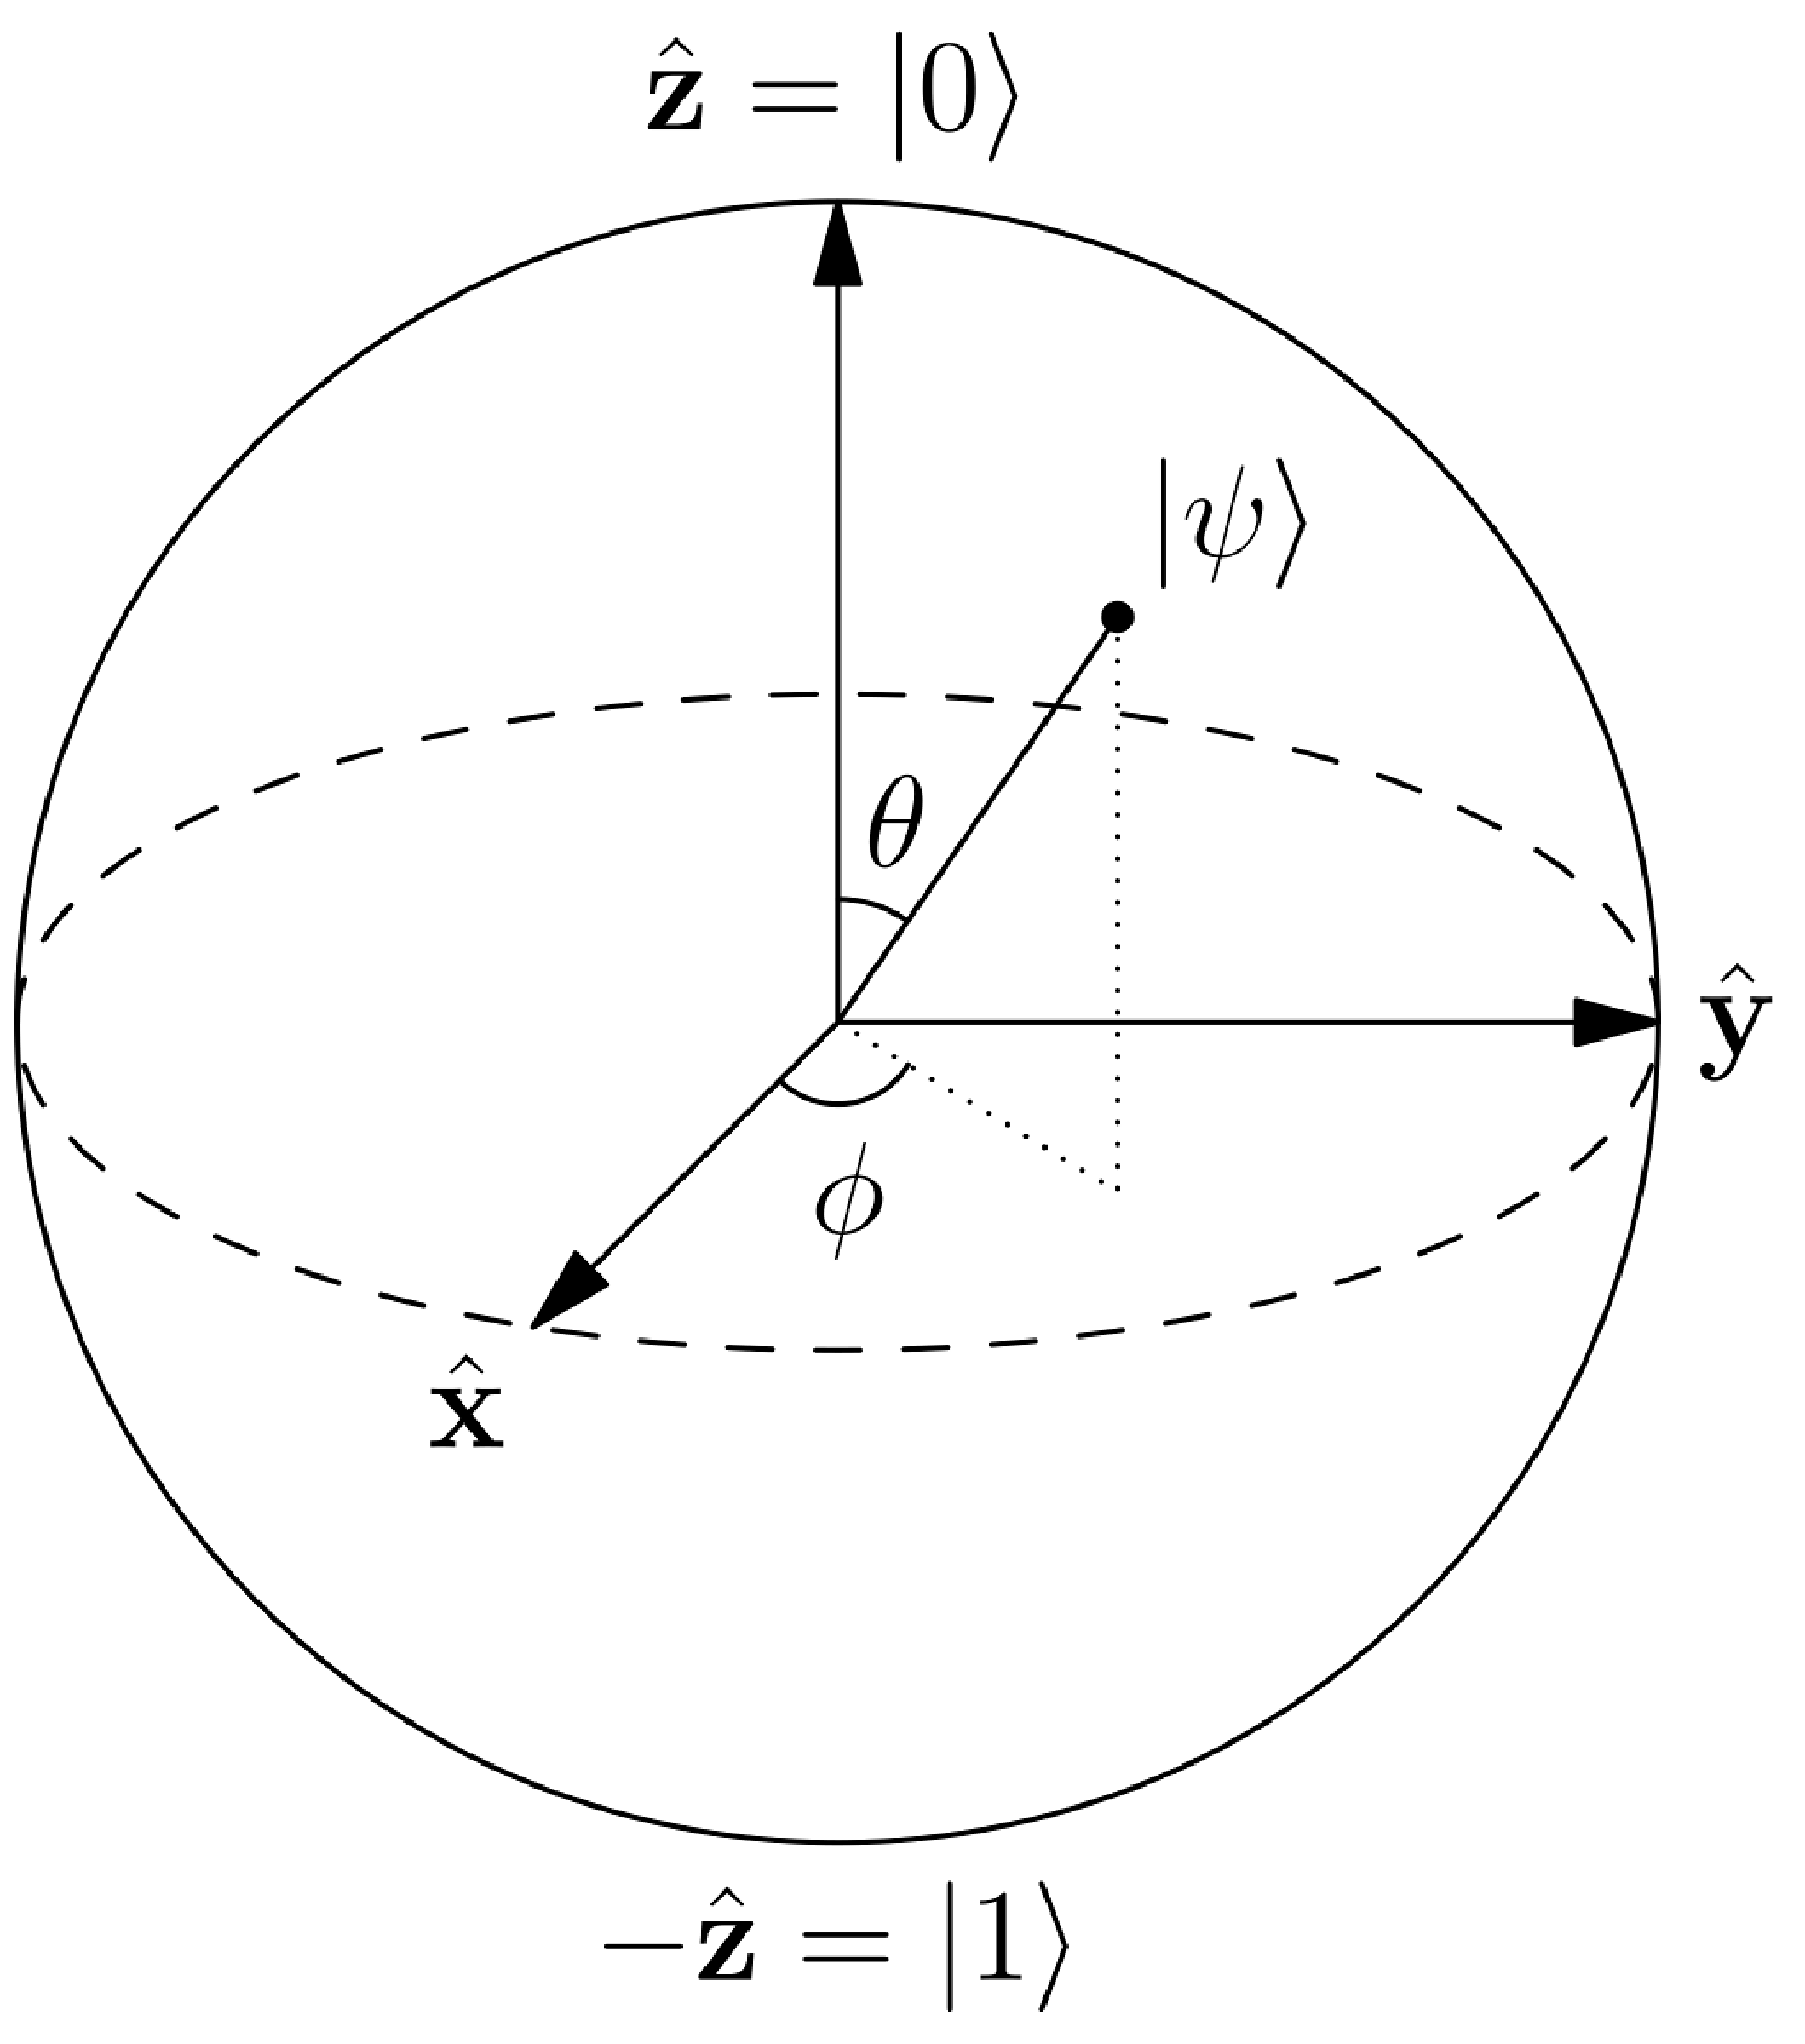
\includegraphics[scale=0.175]{images/bloch_sphere.eps}
  \vspace{2mm}
  \caption{Bloch sphere representation of a qubit.}
  \label{fig:bloch}
\end{figure}

\section{Single-Qubit Quantum Gates}
Single-qubit quantum gates can be seen as counter-clockwise rotations on the Bloch sphere. These gates only have one limitation: they have to be \emph{unitary}, that is $U^\dagger U = UU^\dagger = I$, where $U^\dagger$ is the conjugate transpose of $U$ and $I$ the identity operation. Therefore, any $2^n \times 2^n$ unitary operation is a valid gate which acts on $n$ qubits. We will often use circuit notation to describe a transformation $\ket{\psi'} = U$\ket{\psi} as following:
\[
  \Large
  \Qcircuit @C=1em @R=0em {
    & \lstick{\ket{\psi}} & \gate{U} & \qw & \ket{\psi'}
  }
\]
Below are some notable single-qubit gates described and visualized.

\subsection{Pauli Gates}\label{pauli_gates}
 The most simple quantum gates are the \emph{Pauli gates} $I$, $X$, $Y$ and $Z$. $I$ is the identity gate, which does nothing. The other gates rotate $\pi$ radians (180 degrees) around the X, Y or Z-axis. These gates are self-inverse, meaning $U^2 = I$.

\begin{figure}[ht]
  \centering
  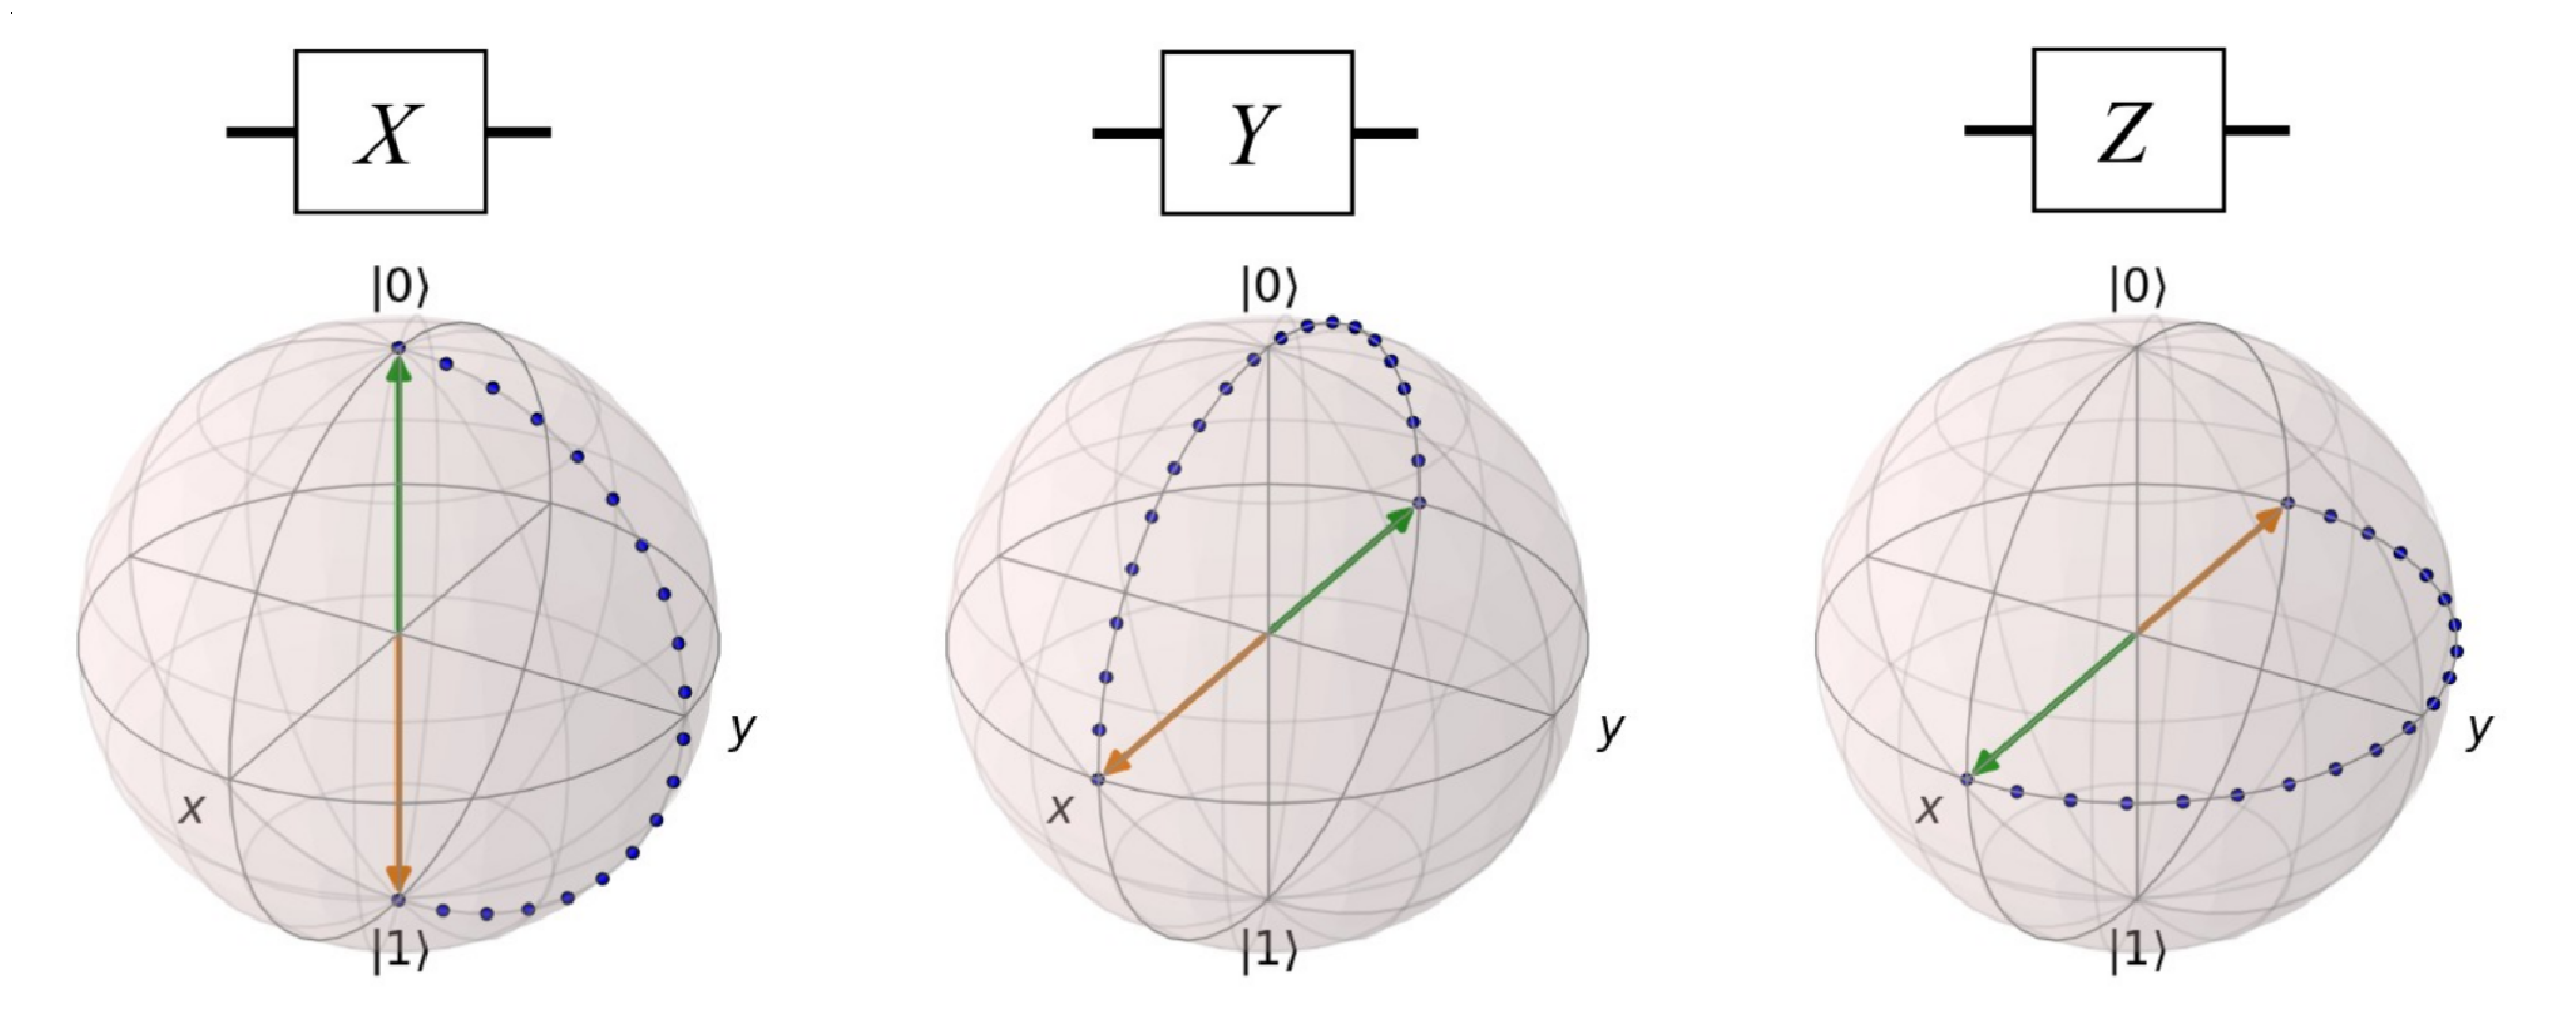
\includegraphics[scale=0.175]{images/pauli_gates.eps}
  \vspace{2mm}
  \caption{Pauli gates $X$, $Y$ and $Z$ visualized on the Bloch sphere. The green vector is the starting position and the orange vector the final position.}
\end{figure}

\subsection{Hadamard Gate}
The \emph{Hadamard} ($H$) gate (Figure \ref{fig:hadamard_bloch}) maps the basis states \ket{0} and \ket{1} to superposition states with equal weight:
\begin{align}
  H\ket{0} &= \dfrac{1}{\sqrt2}(\ket{0} + \ket{1}) = \ket{+} \\
  H\ket{1} &= \dfrac{1}{\sqrt2}(\ket{0} - \ket{1}) = \ket{-}.
\end{align}
It is the combination of two rotations, $\pi$ radians about the Z-axis followed by $\pi/2$ radians about the Y-axis. The Hadamard gate belongs to the Clifford gates.

\begin{figure}[ht]
  \centering
  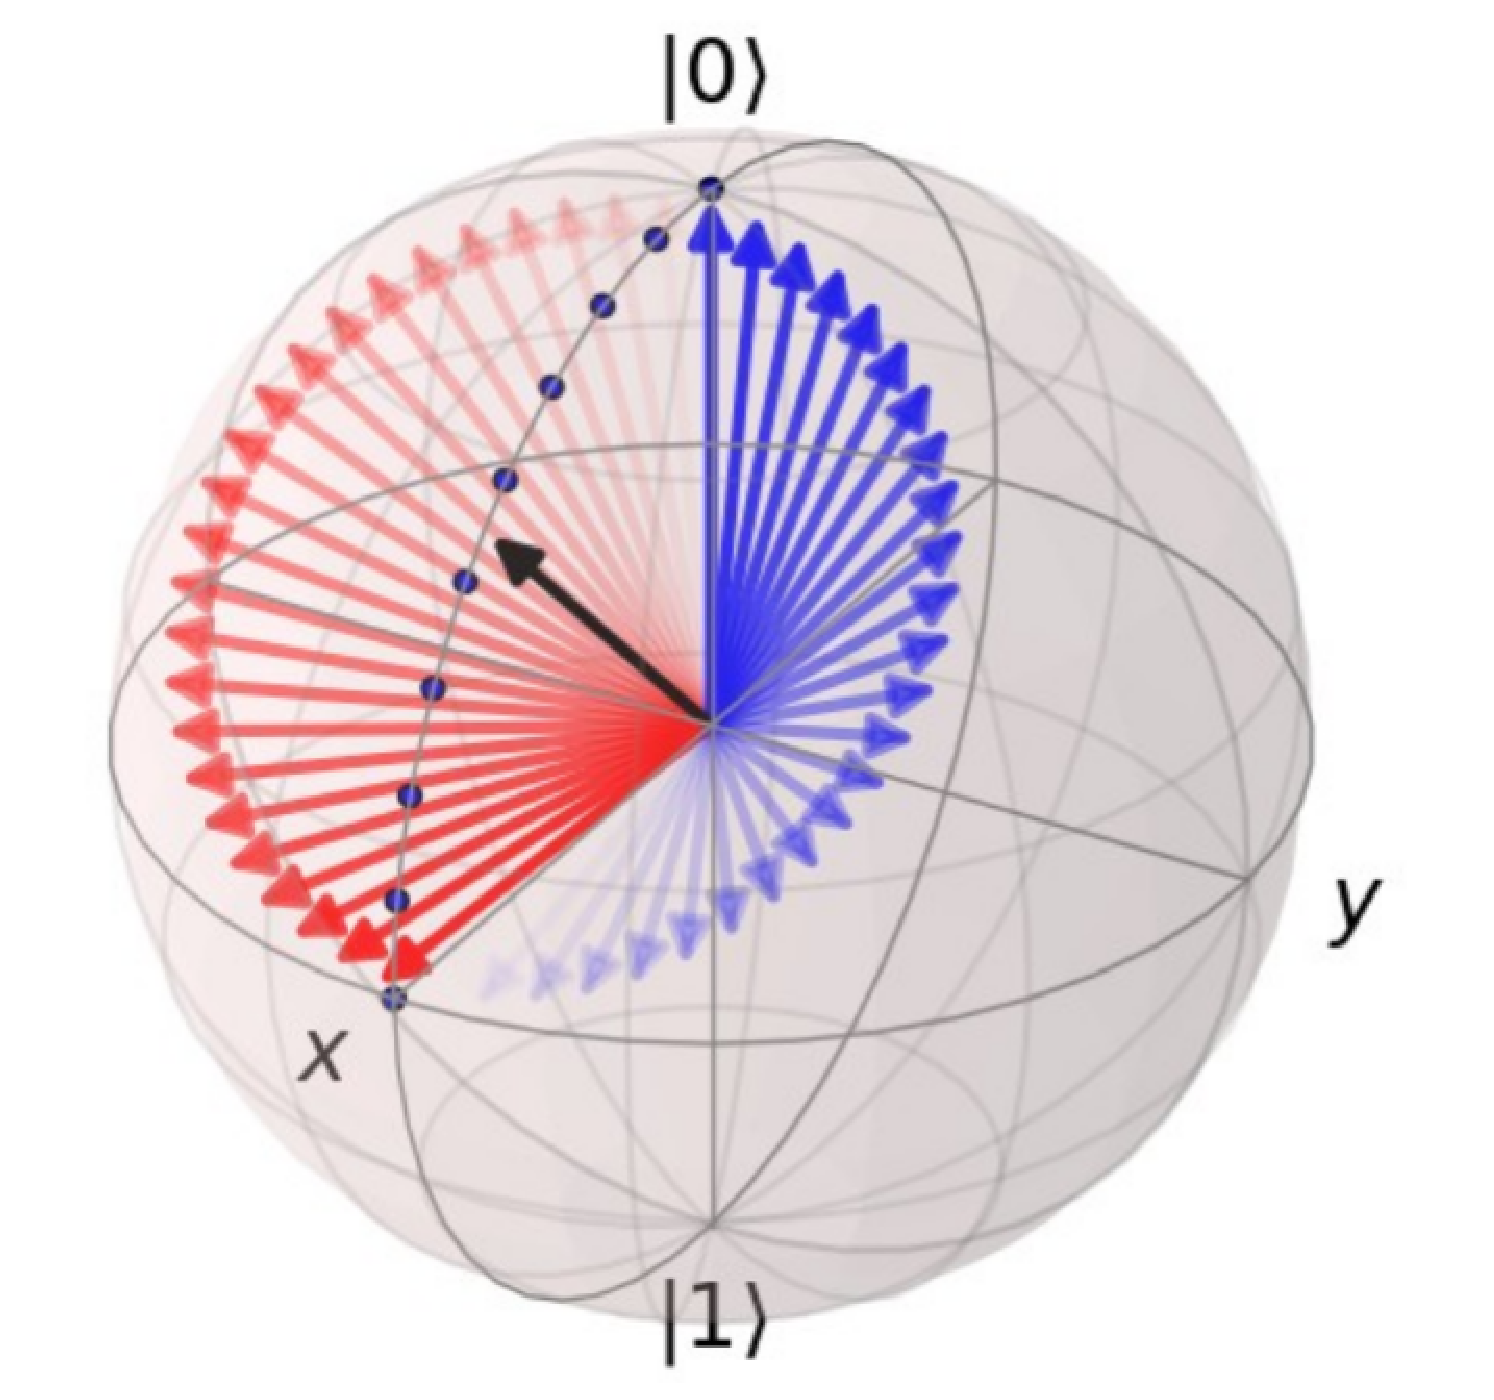
\includegraphics[scale=0.17]{images/hadamard_gate.eps}
  \vspace{1mm}
  \caption{Hadamard gate visualized on the Bloch sphere.}
  \label{fig:hadamard_bloch}
\end{figure}

\subsection{Phase Gates}
Rotation gates that rotate around the Z axis are considered \emph{phase gates}. They rotate the phase of the \ket{1} state by an angle $\theta$ and leave the \ket{0} state unchanged:
\begin{equation}
  \begin{aligned}
    R_z(\theta) \ket{0} &= \ket{0} \\
    R_z(\theta) \ket{1} &= e^{i\theta}\ket{1}.
  \end{aligned}
\end{equation}
The probability of measuring a \ket{0} or \ket{1} is unchanged after a phase gate, however it modifies the phase of the quantum state. A common phase gate is the $S$ gate, where $\theta = \pi/2$ (Figure \ref{fig:s_bloch}). The Pauli Z gate can be thought of as a phase gate where $\theta = \pi$, because $e^{i\pi} = -1$. Thus you could also think of the $S$ gate as half a Pauli $Z$ gate. Another common phase gate is the $T$ gate, where $\theta = \pi/4$ (half an $S$ gate).

\begin{figure}[ht]
  \centering
  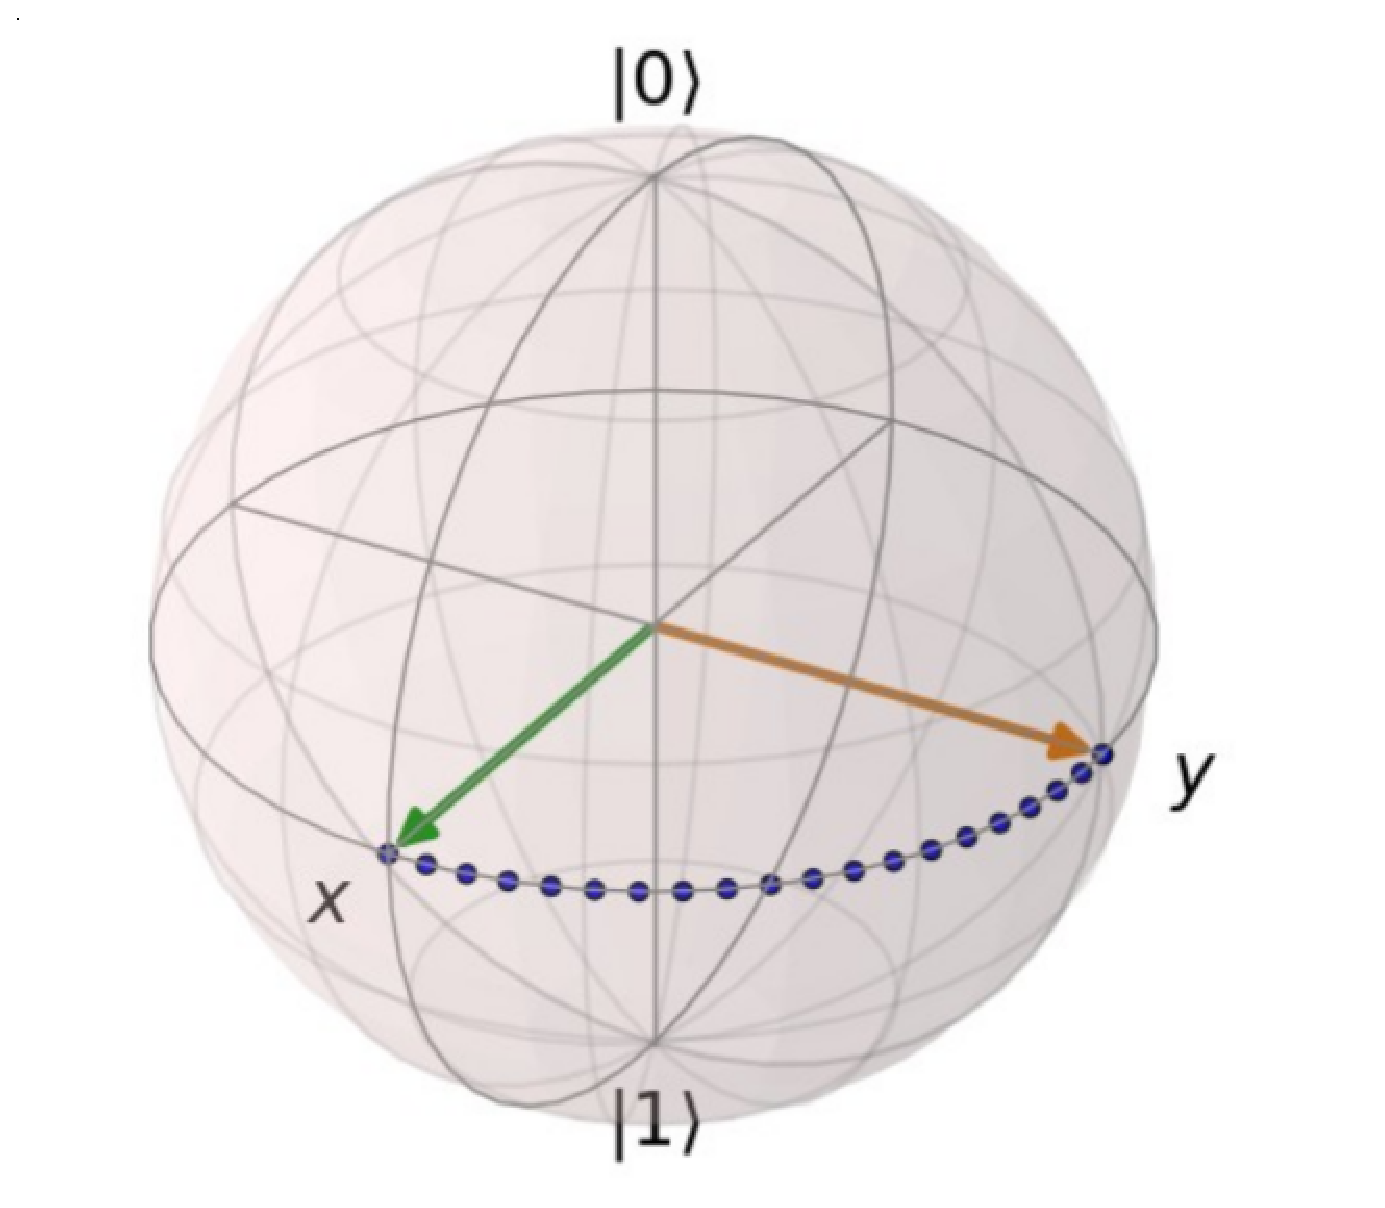
\includegraphics[scale=0.21]{images/s_gate.eps}
  \vspace{1mm}
  \caption{$S$ gate rotation visualized on the Bloch sphere.}
  \label{fig:s_bloch}
\end{figure}

\section{Measurement}
Measuring a quantum state \ket{\psi} in the computational basis \emph{collapses} the quantum superposition to a basis state \ket{j}. The state \ket{\psi} has ``disappeared" and the state is left in \ket{0} or \ket{1}. The probabilistic result of a measurement of a quantum state $\ket{\psi} = \alpha\ket{0} + \beta\ket{1}$ can be calculated based on the probability amplitudes:
\begin{align}
  P(\ket{0}) &= \left|\alpha\right|^2 \\
  P(\ket{1}) &= \left|\beta\right|^2.
\end{align}
Consider the following simple single-qubit circuit:

\begin{figure}[ht]
  \[
    \Large
    \Qcircuit @C=1em @R=0em {
      \push{\rule{0em}{1em}} & & \lstick{\ket{0}} & \gate{H} & \gate{Z} & \meter & \cw
    }
  \]
\caption{A simple quantum circuit. The output of measuring a qubit is a classical bit, which is distinguished from a qubit by drawing a double-line wire. A visualization of this circuit on the Bloch sphere can be seen in Figure~\ref{fig:gate_rotations}.}
\end{figure}
\noindent
We start with computing $H\ket{0} = \ket{+}$, followed by $Z\ket{+} = (\ket{0} - \ket{1})/\sqrt 2$ \, (or \ket{-}). Finally we measure, giving us a computational basis state \ket{j} and collapsing the state. Which state we will see is not determined in advance; the only thing we can say is that we will see \ket{j} with probability $|a_j|^2$:
\begin{align}
  P(\ket{0}) = \left|\dfrac{1}{\sqrt2}\right|^2 &= \dfrac{1}{2} \\
  P(\ket{1}) = \left|\dfrac{-1}{\sqrt2}\right|^2 &= \dfrac{1}{2}.
\end{align}
Giving us equal probabilities of our state being measured as \ket{0} or \ket{1}.

\begin{figure}[ht]
  \centering
  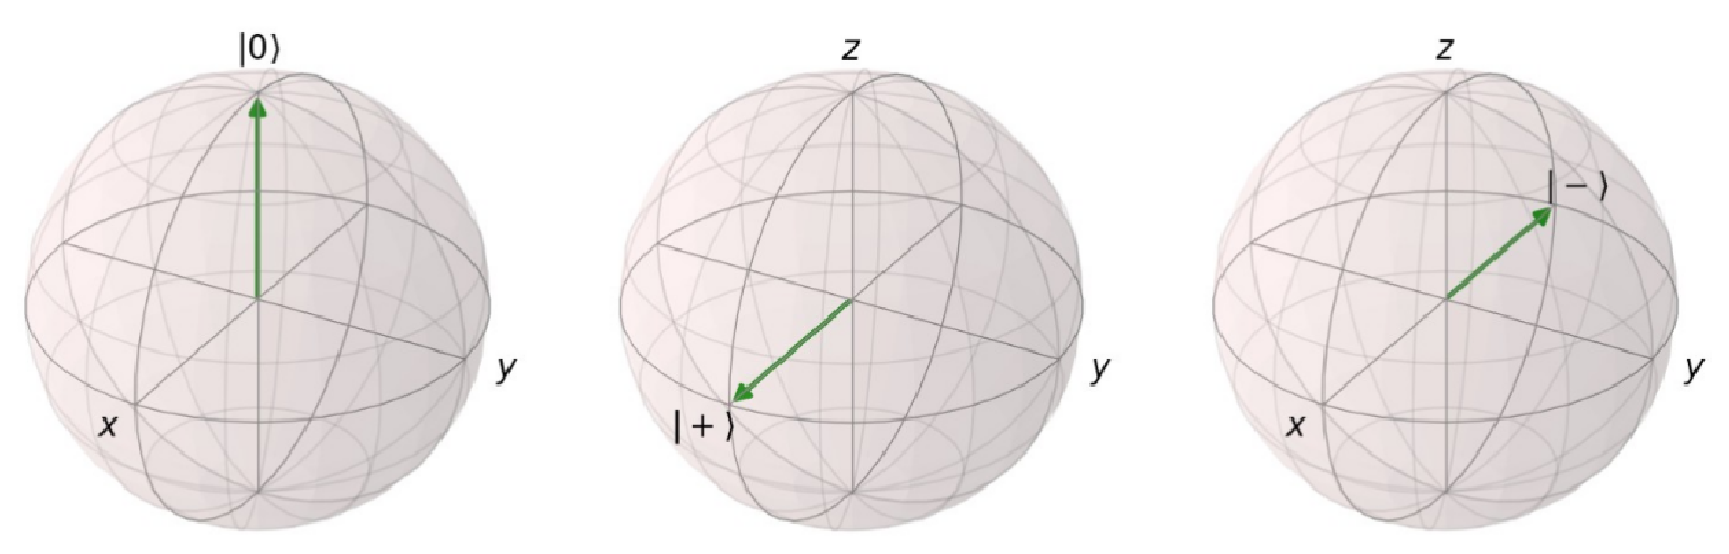
\includegraphics[scale=0.375]{images/simple_circuit.eps}
  \vspace{2mm}
  \caption{States of the qubit throughout the circuit from left to right: \ket{0} $\rightarrow$ $H$\ket{0} $\rightarrow$ $ZH$\ket{0}.}
  \label{fig:gate_rotations}
\end{figure}

\section{Vector Notation} \label{sec:matrix_notation}
Earlier we showed that we can represent a quantum state as
\begin{equation}
  \ket{\psi} = \alpha\ket{0} + \beta\ket{1}.
\end{equation}
The kets \ket{\psi}, \ket{0} and \ket{1} in the formula above represent vectors. We define \ket{0} and \ket{1}, the computational basis states, as following:
\setlength\multicolsep{0pt}
\begin{equation}
  \ket{0} = \qstatezero{}; \quad \ket{1} = \qstateone{}.
\end{equation}
\noindent
A quantum state has to be a normalized vector. In general, a qubit's state is a unit vector in a two-dimensional complex vector space. A $n$ qubit state has a $2^n$ dimensional \emph{Hilbert space}. We can consider a quantum state to be a linear combination of the computational basis states:
\begin{equation}
  \ket{\psi} = \alpha\qstatezero{} + \beta\qstateone{} = \begin{pmatrix}\alpha \\ \beta\end{pmatrix}.
\end{equation}
Single-qubit gates can then be represented by $2 \times 2$ unitary matrices:
\vspace*{-4mm}
\setlength\multicolsep{0pt}
\begin{multicols}{3}
  \[
    I = \igate{};
  \]
  \vfill
  \[
    X = \xgate{};
  \]
  \vfill
  \[
    Y = \ygate{};
  \]
\end{multicols}
\begin{multicols}{3}
  \[
    Z = \zgate{};
  \]
  \vfill
  \[
    S = \sgate{};
  \]
  \vfill
  \[
    H = \hgate{}.
  \]
\end{multicols}
\bigskip
\noindent
Then a computation like $X$\ket{0} can be calculated by matrix vector multiplication:
\begin{equation}
  X\ket{0} = \xgate{} \qstatezero{} = \qstateone{}.
\end{equation}
And we find that $X\ket{0} = \ket{1}$. Or, more general:
\begin{equation}
  X\begin{pmatrix}\alpha \\ \beta\end{pmatrix} = \begin{pmatrix}\beta \\ \alpha\end{pmatrix}.
\end{equation}

You can combine quantum gates by multiplying their matrices. For example, let's verify that the Hadamard gate is self-inverse (that is, applying it twice is equal to doing nothing) by applying it to itself:
\begin{equation}
  H^2 = \hgate{} \hgate{} = \igate{} = I.
\end{equation}
The result is the identity gate, showing that the inverse of $H$ is indeed itself. It is also a \emph{Hermitian matrix}, because it is equal to its own conjugate transpose: $H = H^\dagger$.
